\section{A more convolved example: \acl{CNN}}


\begin{frame}
  \frametitle{\acl{CNN}: Introduction}

  \begin{textblock}{90}(5, 15)
    \begin{itemize}
    \item Introduced in 1989 - 1995
    \item Specialized for image-like structures
    \item Once again roughly biologically inspired
    \item Influential in the rise of deep-learning
    \item Same task than in the previous section
    \end{itemize}
  \end{textblock}
\end{frame}


\begin{frame}[label=CNN_Overview]
  \note{
    \begin{itemize}
    \item Feed-forward
    \item Special layers
    \item Structure of images
    \end{itemize}
  }
  \frametitle{\acl{CNN}: Computation}

  \begin{textblock}{90}(5,10)
    \begin{center}
      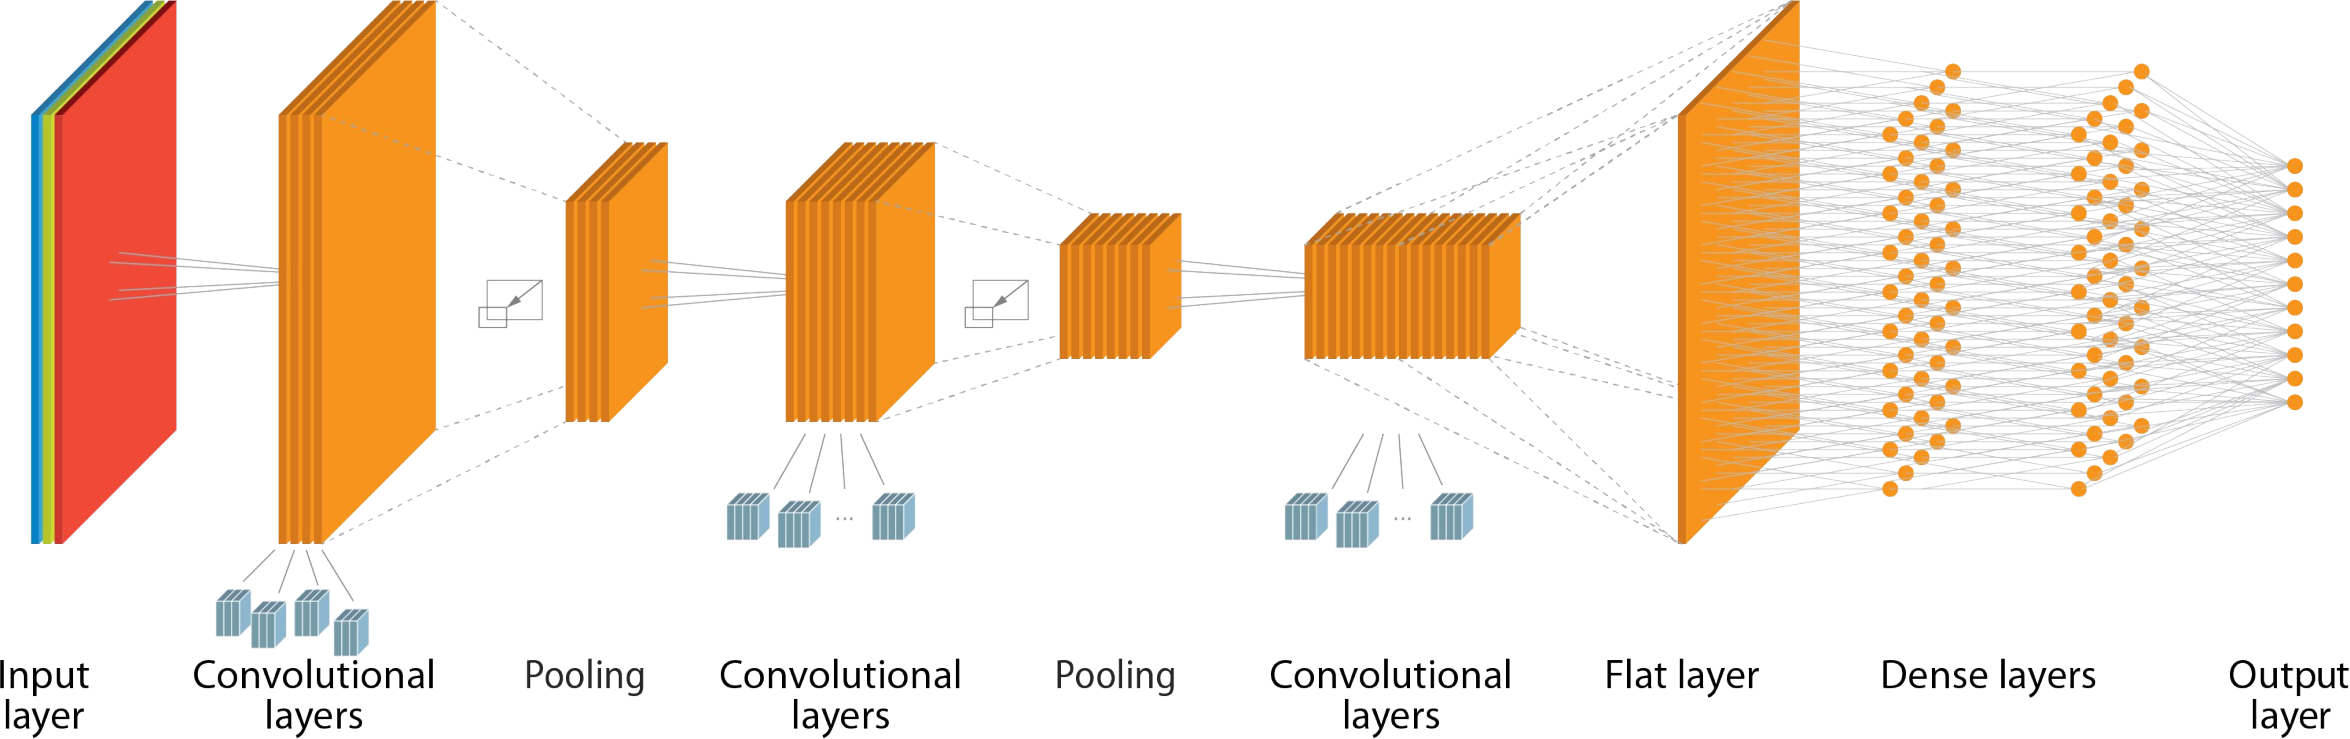
\includegraphics[width=\textwidth]{img/CNN.png}
      Taken from FIDLE
    \end{center}
  \end{textblock}

  \begin{textblock}{45}(5,60)
    \begin{itemize}
    \item Feed-forward architecture
    \item Special layers
      \begin{itemize}
      \item<2-> \hyperlink{Convolutional_Layers}{Convolutional layers}
        \onslide<3->{
          \begin{itemize}
          \item Kernels are learned
          \end{itemize}
        }
      \item<4-> \hyperlink{Pooling_Layers}{Pooling layers}: no weights
      \end{itemize}
    \item<5-> \ac{MLP}
    \end{itemize}
  \end{textblock}

  \begin{textblock}{45}(50,60)
    \onslide<6->{
      \begin{itemize}
      \item The idea is that the layers extract more and more abstract features
      \item Weights are shared: less parameters to learn
      \item Use the \emph{structure} of the image
      \item Many hyper-parameters
      \end{itemize}
    }
  \end{textblock}
\end{frame}


% TODO: hyperlinks
\begin{frame}[label=Convolutional_Layers]
  \frametitle{\acl{CNN}: Convolutional Layers}

  \begin{textblock}{90}(5, 10)
    \begin{center}
      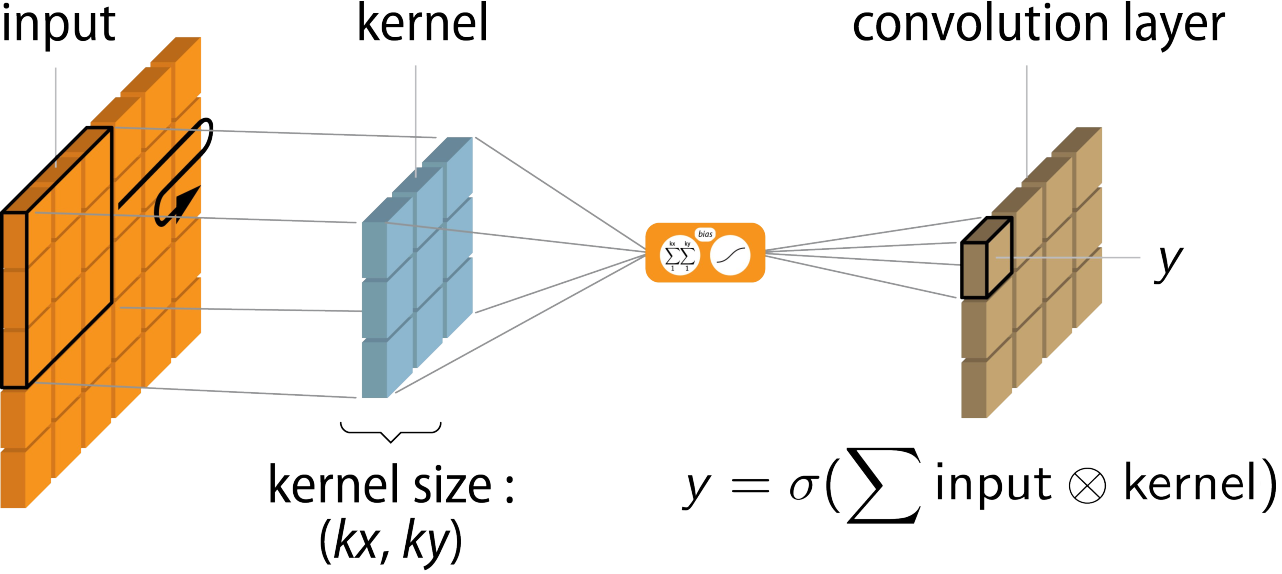
\includegraphics[width=\textwidth]{img/Convolution.png}
      Taken from FIDLE
    \end{center}
  \end{textblock}

  % Cheat a bit on the size
  \begin{textblock}{46}(5, 75)
    \begin{itemize}
    \item Common operation in image processing
    \item $\matrix{K}$ acts as a filter
    \end{itemize}
    %\hyperlink{CNN_Overview}{\beamergotobutton{Go back}}
  \end{textblock}

  \begin{textblock}{45}(50, 75)
    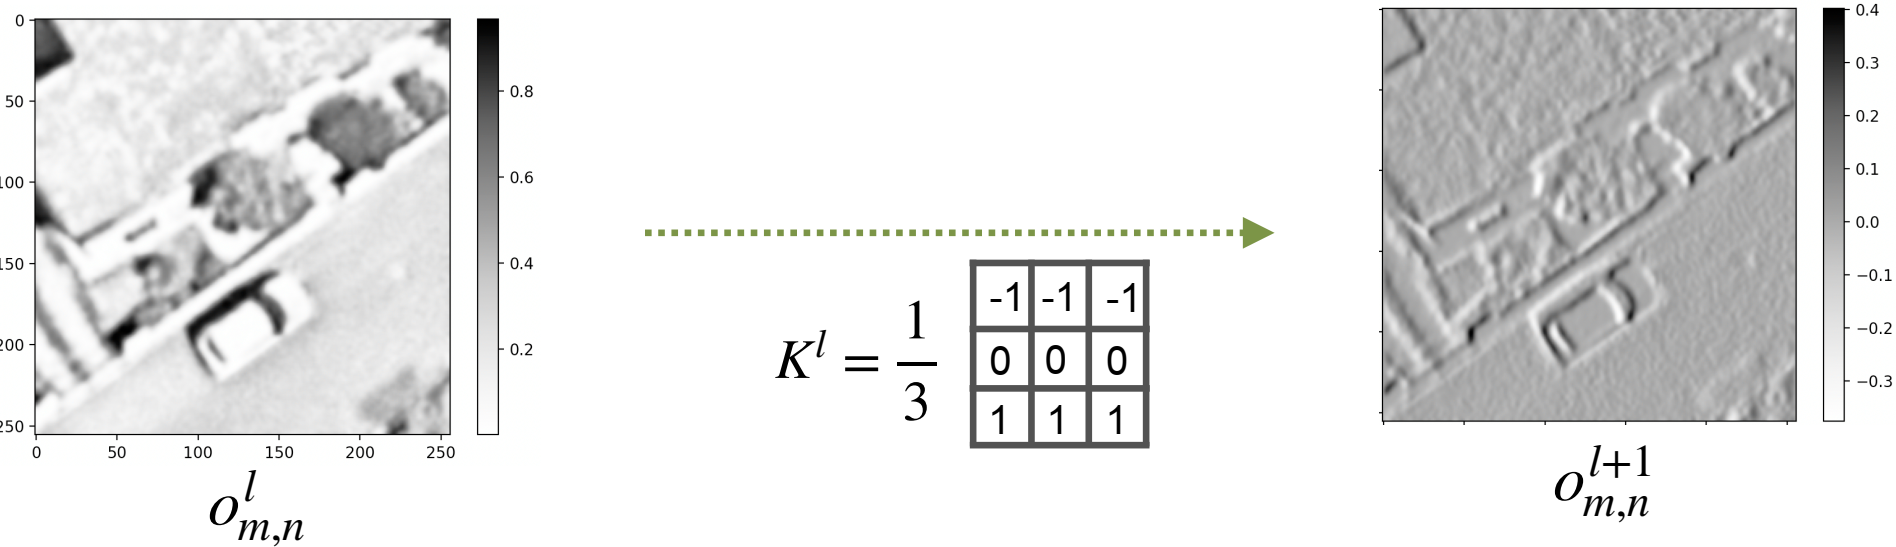
\includegraphics[width=\textwidth]{img/CNN_Filter.png}
  \end{textblock}
\end{frame}


% TODO: hyperlinks
\begin{frame}[label=Pooling_Layers]
  \frametitle{\acl{CNN}: Pooling Layers}

  \begin{textblock}{90}(5, 10)
    \begin{center}
      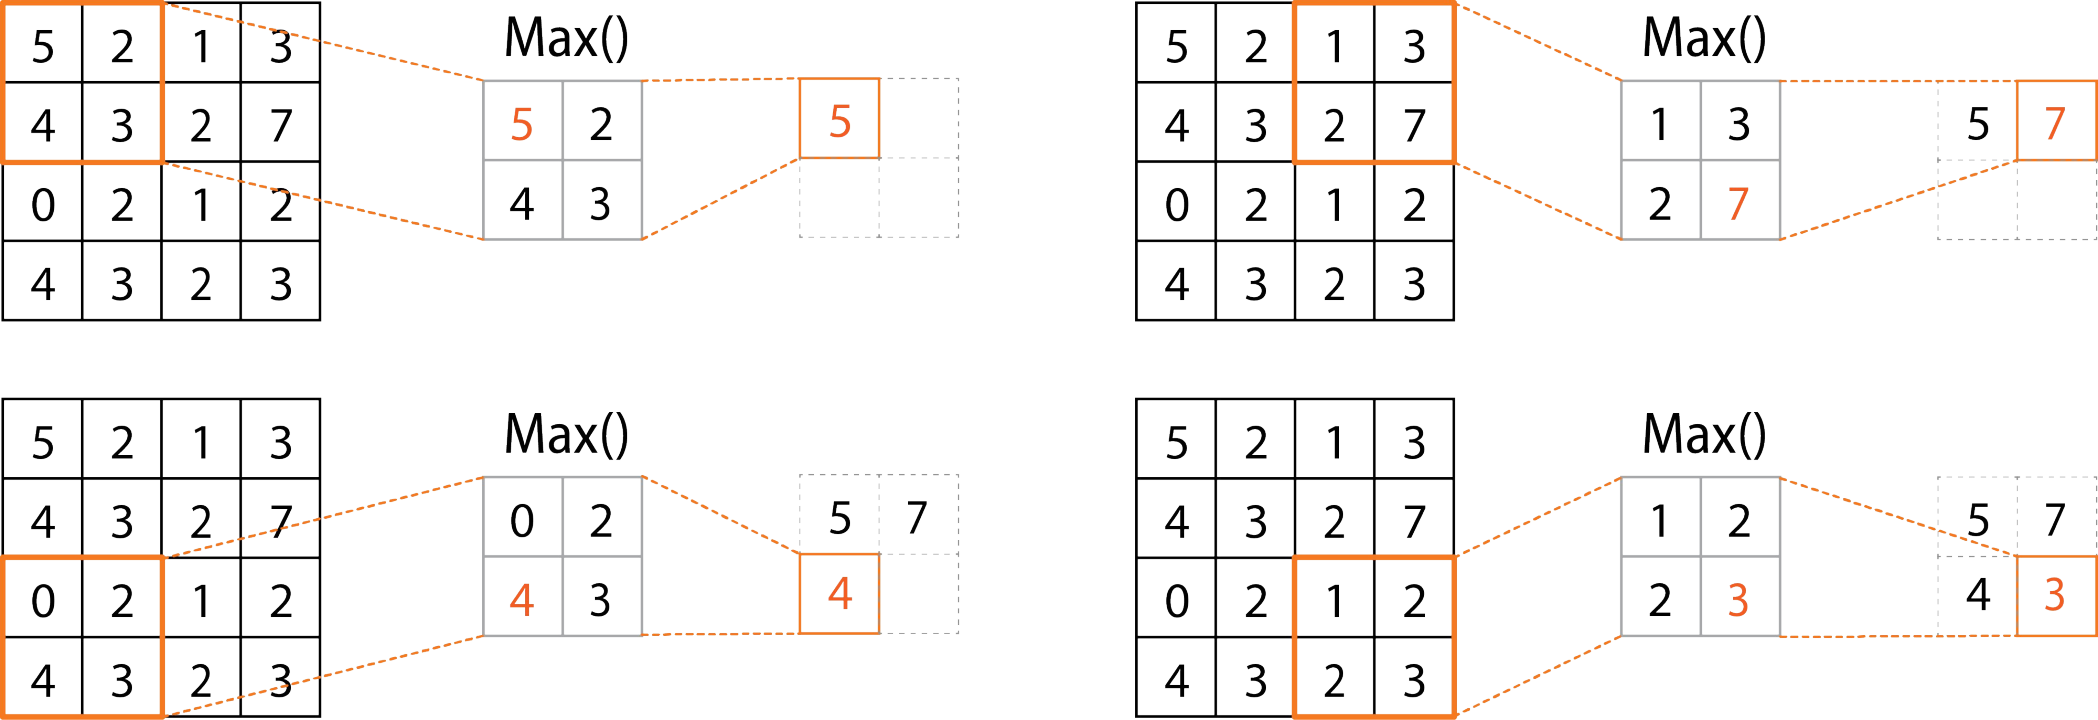
\includegraphics[width=\textwidth]{img/CNN_Pooling.png}
      Taken from FIDLE
    \end{center}
  \end{textblock}

  \begin{textblock}{45}(5, 75)
    Crude downsampling (dimensionality reduction)\\
    %\hyperlink{CNN_Overview}{\beamergotobutton{Go back}}
  \end{textblock}
\end{frame}


\begin{frame}
  \note{
    \begin{itemize}
    \item We can use back-propagation but we must do some computation
    \item Don't present the computation
    \end{itemize}
  }
  \frametitle{\acl{CNN}: Learning}

  \begin{textblock}{90}(5, 15)
    \begin{itemize}
    \item<1-> Same general principle: gradient descent of a loss function
    \item<2-> It's a feed-forward architecture so we know we can use back-propagation
    \item<3-> We have to compute the gradients for convolutional layers!
    \end{itemize}
  \end{textblock}

  \begin{textblock}{90}(5, 30)
    \onslide<4->{
      \begin{center}
        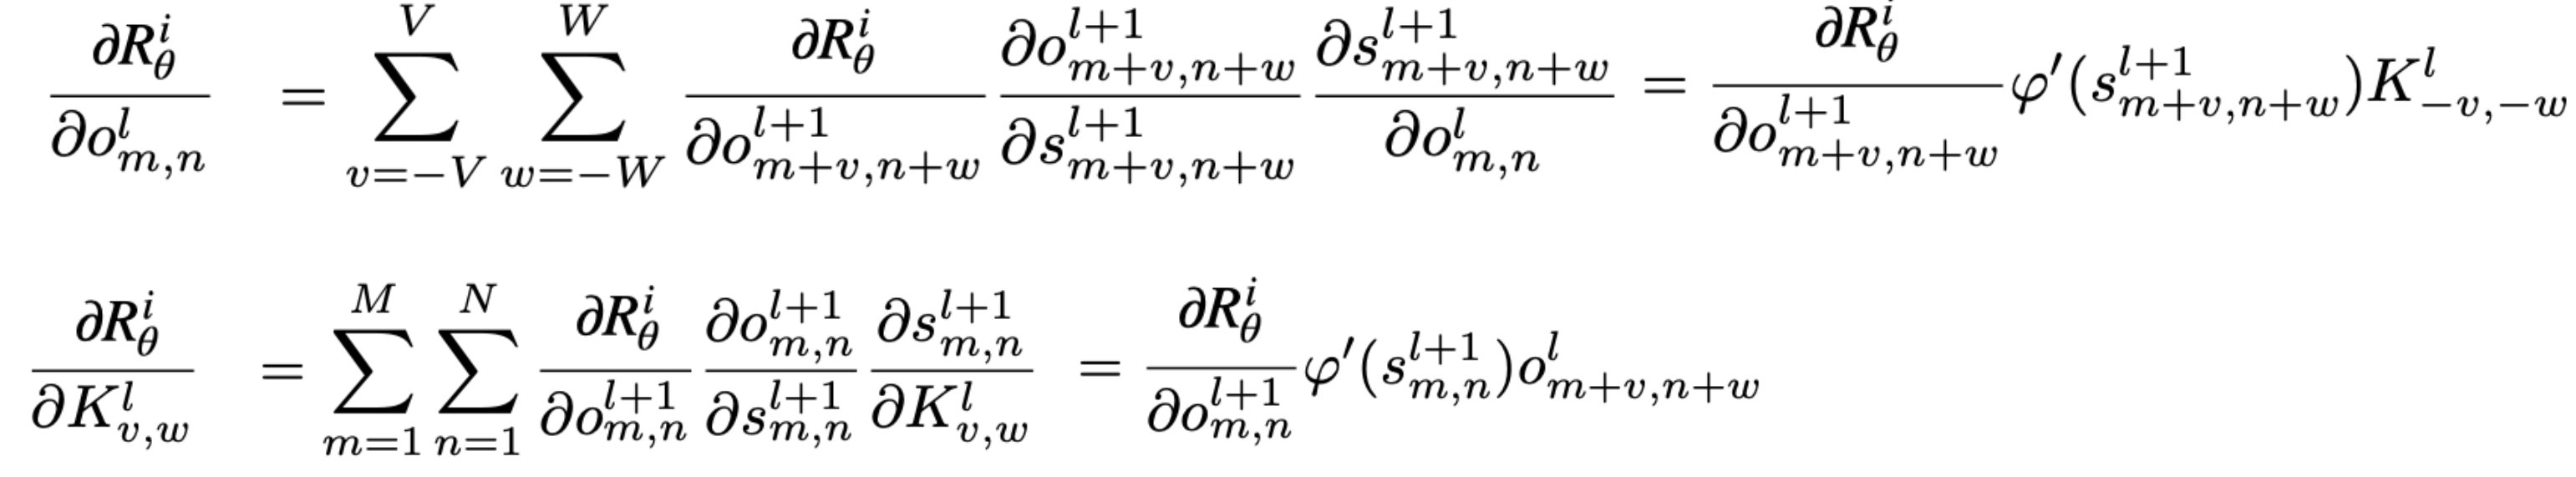
\includegraphics[width=\textwidth]{img/Backpropagation_CNN.png}
      \end{center}
      Taken from FIDLE (notations slightly different ($\varphi \leftrightarrow
      \activFunc$, $R \leftrightarrow \lossFunc$))
    }
  \end{textblock}
\end{frame}


\begin{frame}
  \note{
    \begin{itemize}
    \item Present results:
      \begin{itemize}
      \item 3 times less errors => 3 times less manual intervention when sorting
        letters
      \item Results IRL
      \end{itemize}
    \end{itemize}
  }
  \frametitle{\acl{CNN}: Results}

  \begin{textblock}{90}(5, 15)
    \begin{block}{Results}
      \begin{itemize}
      \item Error rate on MNIST test set $< 1\%$
      \item<2-> Competitive with other methods
      \item<3-> Integrated in some cheque reading systems in 1996
      \item<4-> Much better than \ac{MLP} for other tasks/datasets
      \end{itemize}
    \end{block}
  \end{textblock}

\end{frame}


\begin{frame}
  \note{
    \begin{itemize}
    \item Activation maps are image-like
    \end{itemize}
  }
  \frametitle{\acl{CNN}: Interpretation}

  \begin{textblock}{90}(5, 15)
    \begin{block}{Interpretation}
      \onslide<2->{
        Plot the activations:
        \begin{center}
          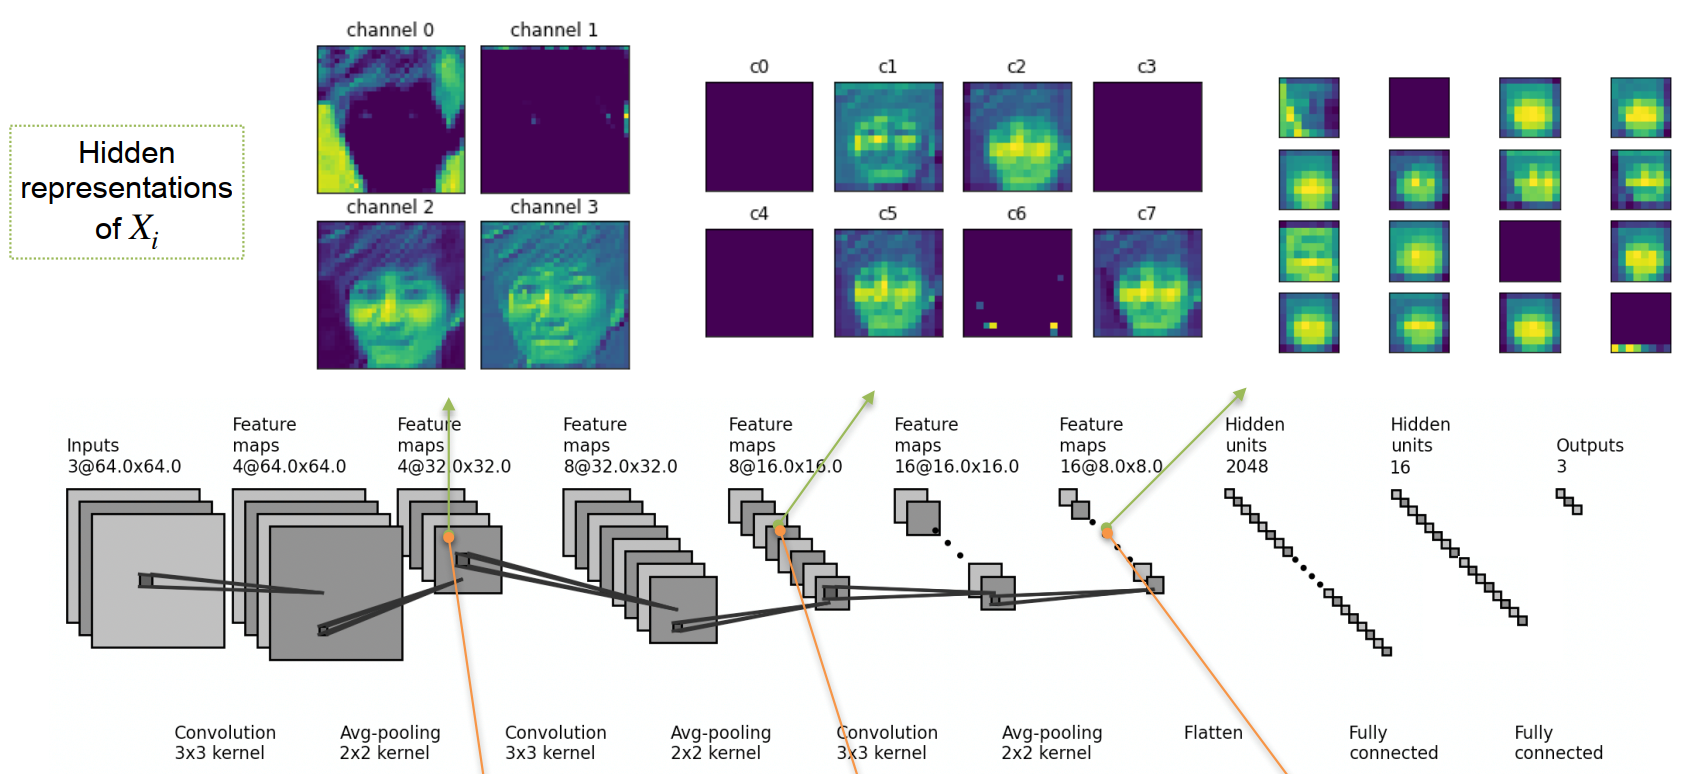
\includegraphics[width=\textwidth]{img/CNN_Interpretation.png}
        \end{center}
        First layers are easier to interpret
      }
      \end{block}
  \end{textblock}

\end{frame}


\begin{frame}
  \frametitle{What have we learned so far?}

  \begin{textblock}{90}(5, 15)
    \begin{itemize}
    \item<1-> No magic!
      \begin{itemize}
      \item YOU have to do the math
      \item YOU have to do the learning, tune the hyper-parameters, \etc{}
      \end{itemize}
    \item<2-> A bit of Neural Networks:
      \begin{itemize}
      \item Neurons: weighted sum and activation function
      \item Architecture: layers and weights
      \item Learning: back-propagation
      \end{itemize}
    \item<3-> Neural networks are very flexible:
      \begin{itemize}
      \item Mathematical foundations are not great, not terrible
      \item Be very careful with biological analogies
      \end{itemize}
    \item<4-> \ac{ML} is not only about models:
      \begin{itemize}
      \item Understand the data to design a model
      \item Need a lot of data \& computational power
      \item Data hell
      \item It's a job!
      \end{itemize}
    \end{itemize}
  \end{textblock}
\end{frame}
